\chapter{Discussion}

In synchrotron X-ray microscopy, the maximal attainable resolution on non-living biological particles is limited to about 10 nm. Unfortunately, synchrotron radiation kills live cells long before any measurable signal can be accumulated, and, as a consequence, no living cell has ever been imaged at high resolution at a synchrotron. ‘Diffraction before destruction’ overcomes this problem and can give high-resolution data, but it only permits one shot from the sample, corresponding to a spherical section through the Fourier amplitudes of the object. Three-dimensional structure determination is possible for identical objects exposed to the beam one-by-one in different orientations; this however cannot be done easily with non-identical objects, such as cells. Methods have been proposed for the simultaneous illumination of cells from multiple directions to provide a 3D view of the object, and instrumentation to achieve this is under development. However, the viewing angles are small and the views one can hope for are few. 

Although 3D imaging would be highly desirable, studies on living cells are based almost entirely on 2D images. Clinical and research laboratories around the world utilize 2D projections of cells. Features are brought out by phase-contrast techniques. We can also do that as described in this thesis.
 
According to predictions, data to sub-nanometer resolution may be recorded on micron-sized living cells through ‘diffraction-before-destruction’. Physical limits to resolution in the pattern are related to sample size and composition, pulse duration, pulse intensity, wavelength and the movement of the sample during exposure. No fundamental limit has been encountered so far with pulses presently available from the LCLS, and the results presented here are in agreement with predictions. It is, however, not trivial to image large objects, like small living cells, at high resolution.

In evaluating resolution we make a distinction between resolution in the signal and in the reconstruction. We have recorded data beyond 4 nm resolution, and reconstructed images up to a resolution of 76 nm. These are still the highest resolution recordings and reconstructions of living cells using coherent diffractive imaging. To reach nanometer resolution in reconstructions, we need to meet certain requirements.

The diffraction signal fades away with an exponent of  about 3.31 over the range of spatial frequencies probed in our measurements. Accurate measurement of nanometer signal requires very low background. Container-free sample injection delivers truly isolated samples into the X-ray beam to record diffraction patterns with low scattered background. Under these conditions, signal from the sample can be measured to the highest possible resolution over a flat background. The contrast between the sample and its surrounding (wet helium gas expanding into a vacuum chamber) is high. The clean background and the high contrast are important for the finite support constraint in phase retrieval. We estimate that nanometer resolution in the signal of a micron-sized cell would require a pulse with duration shorter than 10 fs and around $10^{12}$–$10^{13}$ photons on a micron-sized sample at 3-10 keV photon energy.

Resolution in a 2D reconstruction from a single exposure depends on the success of phase retrieval, and is also influenced by the lift-off of the Ewald sphere from the projection plane at high angles (shorter wavelengths would alleviate this problem). The projection approximation also presumes that the Born approximation is valid. This requires harder X-rays for samples thicker than those studied here.

The maximal size of an object for successful reconstruction is currently limited to about 1-2 micron at the LCLS for a number of reasons. 
First, the bandwidth of an LCLS pulse is about 0.2\% and this gives about 500 resolution elements in an image. If a target resolution of 2 nm is aimed for, the object size cannot be bigger than about 1 micron. Smaller bandwidth would allow studies on larger objects. An oversampled diffraction pattern is necessary for phase retrieval. 
Second, the focus must be large enough to cover the sample yet contain enough photons to produce strong scattered signal from the cell. A larger focus requires more photons per pulse and these extra photons are currently not available from the LCLS. This limits the maximal useful focus size, which in turn limits the object size to about 1-2 micron.

Missing low-resolution data pose perhaps the largest problem in image reconstruction. Low-resolution terms are crucial for the determination of the support for the object. The X-ray detector has a hole at its centre to let the direct beam pass through. The size of this blind spot limits the maximal object size to 1-2 $\mu m$m at the relevant wavelengths. In strong exposures, there is a further and significant loss of low-resolution data due to detector saturation.

The current limitations are technical. A femtosecond exposure ‘freezes’ all cellular processes at room temperature, including diffusion, and thus eliminates blurring. This is an advantage over other cell-imaging methods and will become important if or when nanometer/subnanometer resolution will be achieved on a micron-sized cell. At the moment, the LCLS is still too weak. This is illustrated in Figure \ref{fig:landscape}.


\begin{figure}[!h]
\centering
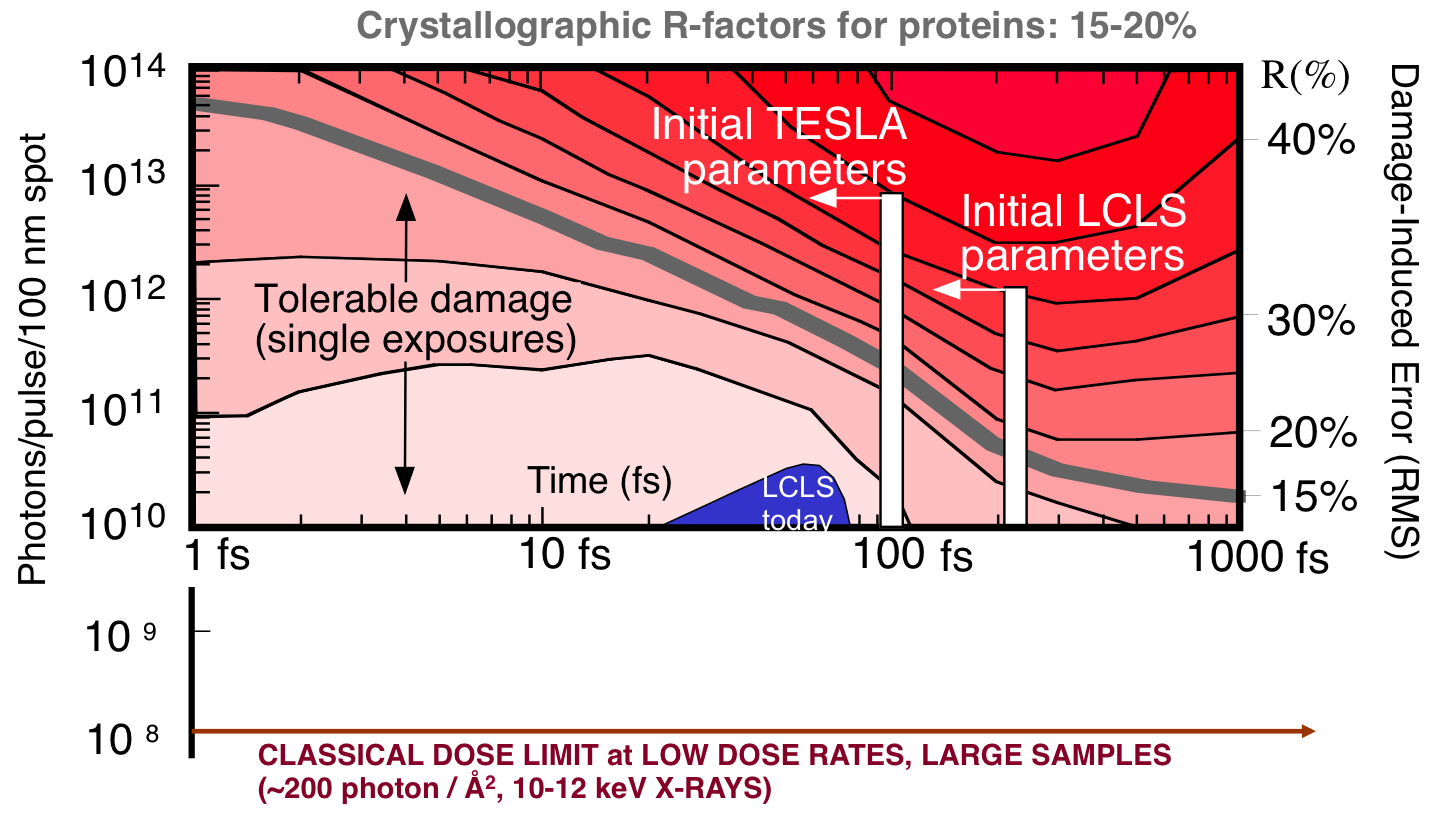
\includegraphics[width=120mm]{Chapter_10_Discussion_LandscapeDamageTolerance.png}
\caption{The landscape of damage tolerance. Contour plots of the weighted electronic R factors [from equation (2) in \cite{Neutze2000}] as functions of the X-ray  flux and pulse duration at 12 keV photon energy. The plot illustrates the extent to which the information content of the elastically scattered X-rays is degraded by radiation damage. Damage as regarded acceptable if the R-factor is below 15\%,  indicated by the grey line. Photon pulses from the LCLS are weak, and have not reached the grey line anywhere in the parameter space.}\label{fig:landscape}
\end{figure}

No fundamental limit has been encountered at free-electron lasers so far, and exciting new science is still to come. Stronger and shorter pulses, like those expected from the European XFEL could bring high-resolution cellular imaging within reach. 
